\documentclass[12pt,a4paper]{article}
\usepackage[utf8]{inputenc}
\usepackage[T1]{fontenc}
\usepackage{geometry}
\usepackage{xcolor}
\usepackage[hidelinks]{hyperref}
\usepackage{listings}
\usepackage{courier}
\usepackage{booktabs}
\usepackage{colortbl}
\usepackage{array}

\geometry{margin=2.5cm}

\title{ESP32 Bluetooth RC Controller\\Main Entry Point Documentation}
\author{Miguel Chip}
\date{\today}

\definecolor{codegray}{rgb}{0.95,0.95,0.95}

% ---------- Colors ----------
\definecolor{arduinoOrange}{HTML}{D35400}   % keywords
\definecolor{arduinoGreen}{HTML}{aba632}    % preprocessor (#include)
\definecolor{arduinoBlue}{HTML}{006699}     % constants
\definecolor{arduinoTeal}{HTML}{00979C}     % strings
\definecolor{arduinoGray}{HTML}{95A5A6}     % comments
\definecolor{arduinoLightGreen}{HTML}{3C9A9A} 
\definecolor{arduinoPurple}{HTML}{8E44AD}
\definecolor{arduinoLineGray}{HTML}{999999}
\definecolor{codegray}{HTML}{F2F2F2}
\definecolor{arduinoDarkGreen}{HTML}{275b60}
\definecolor{tableHeader}{HTML}{D35400} % Arduino orange
\definecolor{rowGray}{gray}{0.95}

\usepackage{tikz}
\usetikzlibrary{arrows.meta, positioning}

\newcommand{\ardfn}[1]{\texttt{\textcolor{arduinoOrange}{#1}}}

\newcommand{\ardfnDG}[1]{\texttt{\textcolor{arduinoTeal}{#1}}}
\newcommand{\ardfnOR}[1]{\texttt{\textcolor{arduinoOrange}{#1}}}
% ---------- Arduino language ----------
\lstdefinelanguage{Arduino}{
	language=C++,
	sensitive=true,
	%	alsoletter={\#, .},
	alsoletter={\#, 1, 2, 3, 4, 5, 6, 7, 8, 9, 0, \<,\>},
	deletekeywords={void,int,float,double,char,bool,short,long,if,extern, typedef, struct, else, sizeof, union,static, while, break, for, const, unsigned, return, switch, case, default, Wire, false},
	morekeywords={},
	morekeywords=[2]{setup, pinMode, digitalWrite, analogRead, digitalRead, delay, loop, Serial.println, Serial,SerialBT, begin, Serial, printf, controlInit, i2cInit,sendI2CTelemetry, handleBluetooth, inputInit, sendTelemetryIfDue, controlUpdate, typedef, struct, sizeof, union, memmove, memcpy, controlHandleEvent, Wire, read, write, endTransmission, requestFrom, beginTransmission, println,available, hasClient,
		inputUpdate, DEVICE_NAME, BLUETOOTH_H, SerialBT.available, SerialBT.read, SerialBT.write, buf, plotNames, sin, cos, ledcAttach, SerialBT.hasClient, map, mapServo, mapMotor,pulse, readIMU, printStatePacket, printEventPacket, printPanelPacket, printIndicatorPacket, printPlotPacket,sendConfigTelemetry},
	morekeywords=[3]{void, INPUT,INPUT_PULLUP, extern, uint16_t, byte, RcPacket, StatePacketUnion, EventPacket,PanelPacket, IndicatorPacket, PlotPacket, I2CPacket, InputPacket,EventPacketUnion, int,float,bool,long,short,const, char,  static, unsigned, uint32_t},
	morekeywords=[4]{\#include,\#define,\#ifdef,\#ifndef,\#endif,\#pragma, if, for, while, else, break, default, return,switch,case},
	morekeywords=[5]{<Arduino.h>, <BluetoothSerial.h>, false, true},
	morekeywords=[6]{__attribute__, packed},
	morekeywords=[7]{RcPacket, StatePacketUnion}
}

% ---------- Arduino style ----------
\lstdefinestyle{arduino}{
	language=Arduino,
	basicstyle=\ttfamily\small,
	tabsize=2,
	keywordstyle=\color{arduinoOrange}\bfseries,
	keywordstyle=[2]\color{arduinoOrange},
	keywordstyle=[3]\color{arduinoLightGreen},
	keywordstyle=[4]\color{arduinoGreen},
	keywordstyle=[5]\color{arduinoDarkGreen},
	keywordstyle=[6]\color{arduinoPurple},
	keywordstyle=[7]\color{arduinoBlue},
	commentstyle=\color{arduinoGray},
	stringstyle=\color{arduinoTeal},
	numbers=none,
	numberstyle=\tiny\color{arduinoLineGray},
	showstringspaces=false,
	literate=%
	{1000}{{{\color{arduinoLightGreen}1000}}}4
	{250}{{{\color{arduinoLightGreen}250}}}3
	{50}{{{\color{arduinoLightGreen}50}}}2
	{115200}{{{\color{arduinoLightGreen}115200}}}6
	%{sendI2CTelemetry}{{{\color{arduinoOrange}sendI2CTelemetry}}}16
	%	{i2cInit}{{{\color{arduinoOrange}i2cInit}}}7
	%	{0}{{{\color{arduinoLightGreen}0}}}1
	%	{1}{{{\color{arduinoLightGreen}1}}}1
	%	{2}{{{\color{arduinoLightGreen}2}}}1
	%	{3}{{{\color{arduinoLightGreen}3}}}1
	%	{4}{{{\color{arduinoLightGreen}4}}}1
	%	{5}{{{\color{arduinoLightGreen}5}}}1
	%	{6}{{{\color{arduinoLightGreen}6}}}1
	%	{7}{{{\color{arduinoLightGreen}7}}}1
	%	{8}{{{\color{arduinoLightGreen}8}}}1
	%	{9}{{{\color{arduinoLightGreen}9}}}1
}

\lstset{language=Arduino, style=arduino}
\begin{document}
\maketitle
\tableofcontents
\newpage
\setlength{\parskip}{6pt}
\setlength{\parindent}{0pt}
\setlength{\tabcolsep}{12pt}
\renewcommand{\arraystretch}{1.5}

% =========================================================
\section{Project Entry File: ESP32\_BT\_Controller.ino}

\subsection{Purpose}
Este archivo es el \textbf{punto de entrada principal} del sistema RC Bluetooth.
No controla directamente motores o sensores.
Solo \textbf{coordina todos los módulos}:

\begin{itemize}
	\item Comunicación Bluetooth
	\item Decodificación de paquetes
	\item Telemetría
	\item Control de hardware
	\item Entradas locales y sensores I2C
\end{itemize}

Este diseño se llama \textbf{arquitectura modular por capas}.
Cada módulo es independiente y más fácil de mantener.

% =========================================================
\subsection{Módulos incluidos}
\begin{lstlisting}
		#include <Arduino.h>
		#include "bluetooth.h"
		#include "packets.h"
		#include "telemetry.h"
		#include "receiver.h"
		#include "debug.h"
		#include "control.h"
		#include "input.h"
		#include "i2c_sensors.h"
	\end{lstlisting}

\subsection*{Descripción de componentes}
\begin{center}
	\rowcolors{2}{arduinoTeal!8}{arduinoOrange!6}
	\renewcommand{\arraystretch}{1.35}
	\setlength{\tabcolsep}{14pt}

	\begin{tabular}{@{} l p{8cm} @{}}
		\rowcolor{arduinoGreen!25}
		\textbf{File}           & \textbf{Purpose}                     \\ \midrule
		\texttt{Arduino.h}      & Core ESP32 and Arduino functions     \\
		\texttt{bluetooth.h}    & Bluetooth SPP and SerialBT setup     \\
		\texttt{packets.h}      & RC data packet structures            \\
		\texttt{telemetry.h}    & Telemetry transmission logic         \\
		\texttt{receiver.h}     & Bluetooth RX and packet decoding     \\
		\texttt{debug.h}        & Serial debugging helpers             \\
		\texttt{control.h}      & Hardware outputs (PWM, motors, LEDs) \\
		\texttt{input.h}        & Local ESP32 inputs                   \\
		\texttt{i2c\_sensors.h} & Sensor bus over I2C                  \\
	\end{tabular}
\end{center}


% =========================================================
\subsection{Setup Function}

\begin{lstlisting}
		void setup() {
			Serial.begin(115200);
			delay(1000);
			Serial.println("Booting...");
			SerialBT.begin(DEVICE_NAME);
			Serial.println("ESP32 Bluetooth Receiver Ready.");
			Serial.printf(
			"Listening for State (%d) and Event (%d)\n", 
			STATE_PACKET_SIZE, EVENT_PACKET_SIZE
			);
			controlInit();
			i2cInit();
		}
	\end{lstlisting}

\subsection*{Resumen operativo}
\begin{itemize}
	\item Inicia la consola USB a 115200 baudios.
	\item Inicia Bluetooth SPP.
	\item Muestra mensajes de diagnóstico.
	\item Inicializa todas las salidas.
	\item Inicializa sensores I2C.
\end{itemize}

% =========================================================
\subsection{Bucle Principal de Ejecución}

\subsection*{Motor de Control en Tiempo Real}

La función \ardfn{loop}\texttt{()} es el motor de ejecución en tiempo real del
controlador RC con ESP32. Se ejecuta de forma continua después de que finaliza
\ardfn{setup}\texttt{()}, y puede ejecutarse miles de veces por segundo.

Esta función sincroniza:

\begin{itemize}
	\item Datos de control recibidos desde la aplicación Android
	\item Salidas físicas (motores, servos, luces, buzzer)
	\item Telemetría enviada de regreso a Android
	\item Entradas locales conectadas al ESP32
	\item Sensores I2C como voltaje, corriente o temperatura
\end{itemize}

Cada tarea está aislada en su propia función para respetar el principio de
\textbf{separación de responsabilidades}. Ninguna función bloquea el sistema
usando retardos (\texttt{delay}), por lo que el controlador se mantiene
siempre responsivo.

\subsection*{Código Fuente}

\begin{lstlisting}
	void loop() {
		handleBluetooth();
		sendTelemetryIfDue();
		controlUpdate();
		inputUpdate();
		sendI2CTelemetry();
	}
\end{lstlisting}

\subsection*{Descripción Línea por Línea}

\begin{enumerate}
	\item  \ardfn{handleBluetooth}\texttt{();}
	
	Lee los bytes entrantes desde el enlace Bluetooth SPP. Esta función
	reconstruye los paquetes enviados por la app Android, valida su
	checksum, identifica si son paquetes de estado o de evento, y actualiza
	las estructuras globales definidas en \texttt{packets.h}.
	
	\item  \ardfn{sendTelemetryIfDue}\texttt{();}
	
	Envía paquetes de telemetría a la aplicación Android solo cuando ha
	transcurrido el intervalo de tiempo definido. Esto evita saturar el
	canal Bluetooth sin perder fluidez en la interfaz.
	
	\item  \ardfn{controlUpdate}\texttt{();}
	
	Convierte las posiciones de los sticks, valores de perillas y estados
	de interruptores en salidas físicas reales. Actualiza los canales PWM
	para motores y servos, y configura salidas digitales para luces,
	relés y dispositivos auxiliares.
	
	\item  \ardfn{inputUpdate}\texttt{();}
	
	Lee entradas locales como botones físicos, potenciómetros o sensores
	digitales conectados al ESP32. Cuando se detecta un cambio, se envía
	un evento a la aplicación Android.
	
	\item  \ardfn{sendI2CTelemetry}\texttt{();}
	
	Lee todos los sensores I2C conectados y empaqueta sus valores en
	tramas de telemetría que se transmiten a la aplicación Android.
\end{enumerate}

\subsection*{Justificación del Orden de Ejecución}

\begin{enumerate}
	\item Recibir primero los datos de control
	\item Transmitir la telemetría
	\item Actualizar las salidas de hardware
	\item Leer las entradas locales
	\item Enviar telemetría de sensores
\end{enumerate}

Este orden garantiza un comportamiento determinista, una respuesta rápida
y un control seguro de los motores.

% =========================================================
\section{Capa de Comunicación Bluetooth}

\subsection{Propósito}

La capa Bluetooth proporciona el enlace de comunicación inalámbrica entre el
controlador ESP32 y la aplicación Android utilizando el
\textbf{Serial Port Profile (SPP)}.

Este módulo:

\begin{itemize}
	\item Crea una interfaz serial Bluetooth global
	\item Define el nombre del dispositivo Bluetooth
	\item Hace que el objeto Bluetooth sea accesible desde todos los módulos
\end{itemize}

No contiene lógica ni procesamiento de datos.
Solo proporciona el canal de comunicación.

\subsection{Estrategia de Diseño}

En lugar de crear múltiples objetos Bluetooth, este sistema utiliza una
\textbf{única instancia global de BluetoothSerial} compartida entre todos
los módulos.

Esto se logra usando la palabra clave \texttt{extern} en el archivo de cabecera
y una única definición en el archivo de implementación.

\subsection{Archivo de Cabecera: \ardfnDG{bluetooth.h}}

\begin{lstlisting}
	#ifndef BLUETOOTH_H
	#define BLUETOOTH_H
	
	#include <BluetoothSerial.h>
	
	extern BluetoothSerial SerialBT;
	
	#define DEVICE_NAME "ESP32-BT"
	
	#endif
\end{lstlisting}

\subsection{Archivo de Implementación: \ardfnDG{bluetooth.cpp}}

\begin{lstlisting}
	#include "bluetooth.h"
	
	BluetoothSerial SerialBT;
\end{lstlisting}

\subsection{Acceso Global al Objeto}

Cualquier módulo que incluya \ardfnDG{bluetooth.h} puede utilizar:

\begin{lstlisting}
	SerialBT.begin(DEVICE_NAME);
	SerialBT.available();
	SerialBT.read();
	SerialBT.write(...);
	SerialBT.hasClient();
\end{lstlisting}

Esto permite una comunicación transparente entre:

\begin{center}
	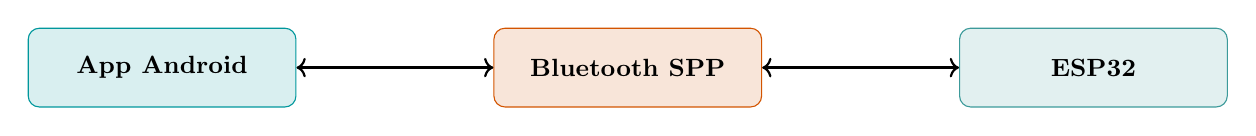
\begin{tikzpicture}[
		node distance=2.5cm,
		every node/.style={
			draw,
			rounded corners=4pt,
			minimum width=3.4cm,
			minimum height=1cm,
			align=center,
			font=\small
		},
		arrow/.style={<->, thick}
		]
		
		\node[fill=arduinoTeal!15, draw=arduinoTeal] (android) {\textbf{App Android}};
		\node[fill=arduinoOrange!15, draw=arduinoOrange, right=of android] (bt) {\textbf{Bluetooth SPP}};
		\node[fill=arduinoLightGreen!15, draw=arduinoLightGreen, right=of bt] (esp) {\textbf{ESP32}};
		
		\draw[arrow] (android) -- (bt);
		\draw[arrow] (bt) -- (esp);
		
	\end{tikzpicture}
\end{center}

\subsection{Descubrimiento del Dispositivo}

El ESP32 se anuncia con el nombre:

\hspace*{2em}\ardfnDG{ESP32-BT}

Este nombre aparece en la lista de dispositivos Bluetooth de Android
e identifica a tu controlador RC.

\subsection{Por Qué Esta Arquitectura Funciona}

\begin{itemize}
	\item Evita múltiples instancias de la pila Bluetooth
	\item Reduce el consumo de memoria
	\item Permite un diseño modular limpio
	\item Mantiene Bluetooth independiente de las capas de lógica
\end{itemize}

\subsection{Flujo de Datos del Sistema}

\begin{center}
	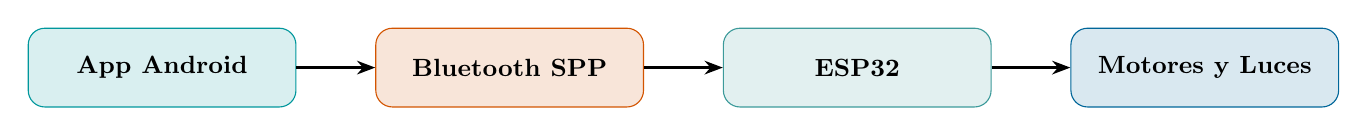
\begin{tikzpicture}[
		node distance=1cm,
		box/.style={
			draw,
			rounded corners=6pt,
			minimum width=3.4cm,
			minimum height=1cm,
			align=center,
			font=\small\bfseries
		},
		arrow/.style={-Stealth, thick}
		]
		
		\node[box, fill=arduinoTeal!15, draw=arduinoTeal] (android) {App Android};
		\node[box, fill=arduinoOrange!15, draw=arduinoOrange, right=of android] (bt) {Bluetooth SPP};
		\node[box, fill=arduinoLightGreen!15, draw=arduinoLightGreen, right=of bt] (esp) {ESP32};
		\node[box, fill=arduinoBlue!15, draw=arduinoBlue, right=of esp] (hw) {Motores y Luces};
		
		\draw[arrow] (android) -- (bt);
		\draw[arrow] (bt) -- (esp);
		\draw[arrow] (esp) -- (hw);
		
	\end{tikzpicture}
\end{center}

\begin{center}
	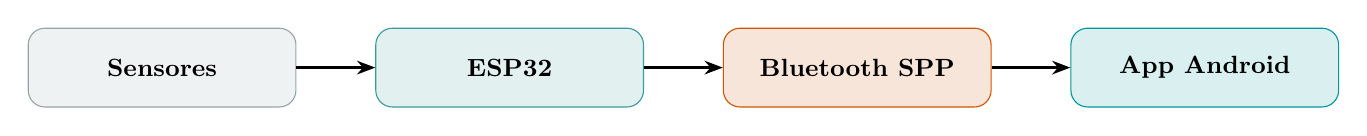
\begin{tikzpicture}[
		node distance=1cm,
		box/.style={
			draw,
			rounded corners=6pt,
			minimum width=3.4cm,
			minimum height=1cm,
			align=center,
			font=\small\bfseries
		},
		arrow/.style={-Stealth, thick}
		]
		
		\node[box, fill=arduinoGray!15, draw=arduinoGray] (sensors) {Sensores};
		\node[box, fill=arduinoLightGreen!15, draw=arduinoLightGreen, right=of sensors] (esp) {ESP32};
		\node[box, fill=arduinoOrange!15, draw=arduinoOrange, right=of esp] (bt) {Bluetooth SPP};
		\node[box, fill=arduinoTeal!15, draw=arduinoTeal, right=of bt] (android) {App Android};
		
		\draw[arrow] (sensors) -- (esp);
		\draw[arrow] (esp) -- (bt);
		\draw[arrow] (bt) -- (android);
		
	\end{tikzpicture}
\end{center}
\section{Capa de Definición de Paquetes}

\subsection{Propósito}

La capa de paquetes define cada mensaje binario que se intercambia entre la
aplicación Android y el controlador ESP32.

Esta capa es la \textbf{única fuente de verdad} para todas las estructuras y
tamaños de comunicación. Todos los demás módulos (\ardfnDG{receiver.cpp},
\ardfnDG{telemetry.cpp}, \ardfnDG{control.cpp}, etc.) dependen de los tipos de
datos declarados aquí.

El sistema de paquetes está diseñado con los siguientes objetivos:

\begin{itemize}
	\item Tramas de tamaño fijo
	\item Bajo consumo de ancho de banda para Bluetooth SPP
	\item Análisis determinista de datos
	\item Uso mínimo de memoria RAM
	\item Verificación rápida de checksum
\end{itemize}

\subsection{Reglas de Diseño}

Todos los paquetes en este sistema siguen las mismas reglas de protocolo:

\begin{itemize}
	\item Cada paquete comienza con dos bytes de cabecera
	\item Cada paquete termina con un byte de verificación (checksum)
	\item Todas las estructuras están marcadas como \texttt{packed} para evitar relleno
	\item Los \textit{unions} permiten acceso como bytes crudos o como estructura
	\item Todos los paquetes están definidos en un único archivo de cabecera
\end{itemize}

\subsection{Archivo de Cabecera: \ardfnDG{packets.h}}

\subsubsection{Paquete de Estado RC}

Este es el paquete principal de control enviado continuamente por la
aplicación Android.

\begin{lstlisting}
	typedef struct __attribute__((packed)) {
		byte startByte1, startByte2;
		uint16_t leftStickX, leftStickY;
		uint16_t rightStickX, rightStickY;
		uint16_t leftKnob, rightKnob;
		byte switches;
		byte checksum;
		byte endByte1, endByte2;
	} RcPacket;
\end{lstlisting}

\paragraph{Campos}

\begin{itemize}
	\item \texttt{startByte1, startByte2} — cabecera fija (sincronización)
	\item \texttt{leftStickX, leftStickY} — dirección y aceleración
	\item \texttt{rightStickX, rightStickY} — paneo auxiliar y segundo motor
	\item \texttt{leftKnob, rightKnob} — controles analógicos para luces y buzzer
	\item \texttt{switches} — interruptores digitales empaquetados en bits
	\item \texttt{checksum} — verificación aditiva
	\item \texttt{endByte1, endByte2} — delimitadores de trama
\end{itemize}

\subsubsection{Contenedor Union}

\begin{lstlisting}
	typedef union {
		RcPacket data;
		byte bytes[sizeof(RcPacket)];
	} StatePacketUnion;
\end{lstlisting}

Esto permite:

\begin{itemize}
	\item \ardfnOR{rcStatePacket}\texttt{.}\ardfnOR{data}\texttt{.}\ardfnOR{leftStickX}
	\item \ardfnOR{rcStatePacket}\texttt{.}\ardfnOR{bytes}\texttt{[i]}
\end{itemize}

\subsubsection{Paquete de Evento}

Los paquetes de evento solo se envían cuando se presiona un botón.

\begin{lstlisting}
	typedef struct __attribute__((packed)) {
		byte startByte1, startByte2;
		byte eventId;
		byte checksum;
	} EventPacket;
\end{lstlisting}

\subsection{Paquetes de Telemetría}

\subsubsection{PanelPacket}

\begin{lstlisting}
	typedef struct __attribute__((packed)) {
		byte header1, header2;
		uint16_t leftPanelValue, rightPanelValue;
		byte panelStates;
		byte checksum;
	} PanelPacket;
\end{lstlisting}

Se utiliza para transmitir valores de indicadores del panel.

\subsubsection{IndicatorPacket}

\begin{lstlisting}
	typedef struct __attribute__((packed)) {
		byte header1, header2;
		byte analogValue, batteryLevel;
		byte checksum;
	} IndicatorPacket;
\end{lstlisting}

Se utiliza para pequeños indicadores visuales.

\subsubsection{PlotPacket}

\begin{lstlisting}
	typedef struct __attribute__((packed)) {
		byte header1, header2;
		byte numPlots;
		byte plotValue1, plotValue2, plotValue3;
		byte checksum;
	} PlotPacket;
\end{lstlisting}

Se utiliza para gráficas de señales en tiempo real.

\subsection{Paquete de Telemetría de Entradas}

Este paquete reporta las entradas físicas conectadas directamente al ESP32.

\begin{lstlisting}
	typedef struct {
		byte h1;
		byte h2;
		uint16_t a34;
		uint16_t a35;
		uint16_t a36;
		uint16_t a39;
		byte d0;
		byte d16;
		byte d17;
		byte checksum;
	} InputPacket;
\end{lstlisting}

Los canales analógicos provienen de GPIO34, 35, 36 y 39.  
Las entradas digitales provienen de GPIO0, 16 y 17.

\subsection{Paquete de Sensores I2C}

\begin{lstlisting}
	typedef struct {
		byte h1;
		byte h2;
		uint16_t temp;
		uint16_t ax;
		uint16_t ay;
		uint16_t az;
		byte sensorFlags;
		byte checksum;
	} I2CPacket;
\end{lstlisting}

Se utiliza para sensores como sondas de temperatura e IMUs.

\subsection{Instancias Globales de Paquetes}

Como los archivos de cabecera no deben reservar memoria, todos los paquetes
globales se definen dentro de \ardfnDG{packets.cpp}.

\begin{lstlisting}
	StatePacketUnion rcStatePacket;
	EventPacketUnion rcEventPacket;
	PanelPacket panelPacket;
	IndicatorPacket indicatorPacket;
	PlotPacket plotPacket;
	InputPacket inputPacket;
	I2CPacket i2cPacket;
\end{lstlisting}

\subsection{Constantes de Tamaño de Paquetes}

Cada paquete tiene un tamaño constante exportado para validación y análisis:

\begin{lstlisting}
	const int STATE_PACKET_SIZE;
	const int EVENT_PACKET_SIZE;
	const int PANEL_PACKET_SIZE;
	const int INDICATOR_PACKET_SIZE;
	const int PLOT_PACKET_SIZE;
\end{lstlisting}

\section{Capa de Recepción Bluetooth}

\subsection{Propósito}

La Capa de Recepción Bluetooth es responsable de convertir un flujo continuo y
no estructurado de bytes Bluetooth en paquetes de control válidos.

Este módulo es la \textbf{puerta de entrada} del sistema.
Cada comando proveniente de la aplicación Android debe pasar por esta capa
antes de poder afectar motores, servos, LEDs o telemetría.

\subsection{Responsabilidades}

El subsistema receptor realiza las siguientes tareas:

\begin{itemize}
	\item Leer bytes crudos desde Bluetooth SPP
	\item Almacenarlos en un buffer circular
	\item Buscar cabeceras de paquetes válidas
	\item Extraer paquetes completos
	\item Copiar los bytes en \textit{unions} estructurados
	\item Llamar a funciones de depuración visual
	\item Disparar eventos de control
\end{itemize}

\subsection{Archivo de Cabecera: \ardfnDG{receiver.h}}

\begin{lstlisting}
	#ifndef RECEIVER_H
	#define RECEIVER_H
	void handleBluetooth();
	#endif
\end{lstlisting}

\paragraph{Descripción}

\begin{itemize}
	\item Declara una única función pública: \ardfnOR{handleBluetooth}\texttt{()}
	\item Esta función se llama continuamente desde el \texttt{loop()}
	\item No devuelve datos: actualiza estructuras globales de paquetes
\end{itemize}

\subsection{Archivo Fuente: \ardfnDG{receiver.cpp}}

\subsubsection{Inclusiones}

\begin{lstlisting}
	#include <Arduino.h>
	#include "bluetooth.h"
	#include "packets.h"
	#include "receiver.h"
	#include "debug.h"
	#include "control.h"
\end{lstlisting}

Estos archivos proporcionan:

\begin{itemize}
	\item El flujo Bluetooth (\texttt{SerialBT})
	\item Definiciones de paquetes
	\item Funciones de depuración
	\item Enlaces con la capa de control
\end{itemize}

\subsubsection{Buffer de Recepción}

\begin{lstlisting}
	#define RX_BUFFER_SIZE 64
\end{lstlisting}

Este buffer es intencionalmente más grande que cualquier paquete.
Permite al sistema sobrevivir a:

\begin{itemize}
	\item Paquetes fragmentados
	\item Múltiples paquetes en una sola ráfaga
	\item Ruido o flujos desalineados
\end{itemize}

\subsubsection{Función Principal: handleBluetooth()}

\begin{lstlisting}[escapeinside={(*@}{@*)},]
	void handleBluetooth() {
		static byte (*@\textcolor{arduinoOrange}{buffer}@*)[RX_BUFFER_SIZE];
		static int bytesRead = 0;
	}
\end{lstlisting}

\paragraph{¿Por qué static?}

\begin{itemize}
	\item El buffer debe conservar su contenido entre iteraciones del \texttt{loop()}
	\item Los paquetes Bluetooth pueden llegar lentamente o por partes
\end{itemize}

\subsubsection{Lectura de Bytes Entrantes}

\begin{lstlisting}[escapeinside={(*@}{@*)},]
	while (SerialBT.available()) {
		if (bytesRead < RX_BUFFER_SIZE) {
			(*@\textcolor{arduinoOrange}{buffer}@*)[bytesRead++] = SerialBT.read();
		} else {
			memmove(buffer, buffer + 1, RX_BUFFER_SIZE - 1);
			(*@\textcolor{arduinoOrange}{buffer}@*)[RX_BUFFER_SIZE - 1] = SerialBT.read();
		}
	}
\end{lstlisting}

Esta lógica:

\begin{itemize}
	\item Agrega nuevos bytes hasta llenar el buffer
	\item Si está lleno, descarta el byte más antiguo
	\item Siempre conserva los datos más recientes
\end{itemize}

\subsubsection{Búsqueda de Paquetes}

\paragraph{Detección de Paquete de Estado}\mbox{}

\begin{lstlisting}[escapeinside={(*@}{@*)},]
	for (int i = 0; i <= bytesRead - 2; i++) {
		if ((*@\textcolor{arduinoOrange}{buffer}@*)[i] == 0xAA &&
		(*@\textcolor{arduinoOrange}{buffer}@*)[i + 1] == 0x55) {
			if (bytesRead - i >= STATE_PACKET_SIZE) {
				packetStart = i;
				packetType = 1;
				break;
			}
		}
	}
\end{lstlisting}

Este bucle escanea el buffer buscando cabeceras válidas.

\paragraph{Detección de Paquete de Evento}\mbox{}

\begin{lstlisting}[escapeinside={(*@}{@*)},]
	if ((*@\textcolor{arduinoOrange}{buffer}@*)[i] == 0xBB &&
	(*@\textcolor{arduinoOrange}{buffer}@*)[i + 1] == 0x66) {
		if (bytesRead - i >= EVENT_PACKET_SIZE) {
			packetStart = i;
			packetType = 2;
			break;
		}
	}
\end{lstlisting}

\subsubsection{Extracción del Paquete}

\begin{lstlisting}[escapeinside={(*@}{@*)},]
	memcpy((*@\textcolor{arduinoOrange}{rcStatePacket}@*).(*@\textcolor{arduinoOrange}{bytes}@*),&(*@\textcolor{arduinoOrange}{buffer}@*)[packetStart],STATE_PACKET_SIZE);
\end{lstlisting}

Esto copia los bytes crudos al \textit{union}, haciendo que los campos
estructurados estén disponibles de inmediato.

\subsubsection{Disparo de Evento}

\begin{lstlisting}[escapeinside={(*@}{@*)},]
	controlHandleEvent((*@\textcolor{arduinoOrange}{rcEventPacket}@*).(*@\textcolor{arduinoOrange}{data}@*).(*@\textcolor{arduinoOrange}{eventId}@*));
\end{lstlisting}

Esto genera inmediatamente la salida de hardware definida en la capa de control.

\subsubsection{Limpieza del Buffer}

\begin{lstlisting}
	memmove(buffer, buffer + removeCount, bytesRead - removeCount);
	bytesRead -= removeCount;
\end{lstlisting}

Esto elimina el paquete procesado y desplaza los bytes restantes.

\subsection{Por Qué un Buffer Circular es Crítico}

Sin un buffer circular, la fragmentación Bluetooth corrompería los paquetes.
Este diseño garantiza:

\begin{itemize}
	\item Ninguna pérdida de bytes
	\item Sin desincronización
	\item Control continuo en tiempo real
\end{itemize}

\section{Capa de Transmisión de Telemetría}

\subsection{Propósito}

El módulo de telemetría es responsable de enviar datos estructurados del sistema
desde el ESP32 hacia la aplicación Android a través de Bluetooth.

A diferencia del módulo receptor, este subsistema es \textbf{solo de escritura}.
Nunca interpreta bytes entrantes. Su única función es:

\begin{itemize}
	\item Construir paquetes de telemetría
	\item Codificar valores del sistema en tiempo real
	\item Calcular sumas de verificación (checksums)
	\item Enviar flujos de bytes crudos
	\item Regular los tiempos de transmisión
\end{itemize}

\subsection{Canales de Paquetes}

Cada mensaje de telemetría comienza con el encabezado común \texttt{0xCC}
y un identificador de tipo:

\begin{center}
	\rowcolors{2}{arduinoTeal!8}{arduinoOrange!6}
	\renewcommand{\arraystretch}{1.4}
	\setlength{\tabcolsep}{14pt}
	
	\begin{tabular}{@{} c c l @{}}
		\rowcolor{arduinoGreen!25}
		\textbf{Encabezado} & \textbf{Tipo} & \textbf{Descripción} \\ \midrule
		\texttt{0xCC} & \texttt{0x11} & PanelPacket \\
		\texttt{0xCC} & \texttt{0x22} & IndicatorPacket \\
		\texttt{0xCC} & \texttt{0x33} & PlotPacket \\
		\texttt{0xCC} & \texttt{0x44} & ConfigPacket (longitud variable) \\
	\end{tabular}
\end{center}

\subsection{Archivo de Cabecera: \ardfnDG{telemetry.h}}

\begin{lstlisting}
	#ifndef TELEMETRY_H
	#define TELEMETRY_H
	void sendTelemetryIfDue();
	void sendConfigTelemetry();
	#endif
\end{lstlisting}

\paragraph{Descripción}

\begin{itemize}
	\item \ardfnOR{sendTelemetryIfDue}\texttt{()} envía paquetes periódicos
	\item \ardfnOR{sendConfigTelemetry}\texttt{()} envía datos de configuración de longitud variable
\end{itemize}

\subsection{Archivo Fuente: \ardfnDG{telemetry.cpp}}

\subsubsection{Inclusiones}

\begin{lstlisting}
	#include <Arduino.h>
	#include <math.h>
	#include "bluetooth.h"
	#include "packets.h"
	#include "telemetry.h"
\end{lstlisting}

\subsubsection{Estado de Temporización}

\begin{lstlisting}
	static unsigned long lastPanelSend = 0;
	static unsigned long lastIndicatorSend = 0;
	static unsigned long lastPlotSend = 0;
\end{lstlisting}

Cada variable almacena el instante de la última transmisión de cada tipo de paquete.

\subsubsection{Intervalos de Transmisión}

\begin{lstlisting}
	const long panelInterval = 1000;
	const long indicatorInterval = 250;
	const long plotInterval = 50;
\end{lstlisting}

\begin{itemize}
	\item Panel: una vez por segundo
	\item Indicador: cuatro veces por segundo
	\item Gráfica: veinte veces por segundo
\end{itemize}

\subsubsection{Metadatos de Gráficas}

\begin{lstlisting}
	const char* plotNames[] = {"Volts","Amps","RPMs"};
	const int NUM_PLOT_NAMES = 3;
\end{lstlisting}

Estas cadenas se envían a la interfaz Android para rotular las gráficas.

\subsection{Paquete de Configuración}

\begin{lstlisting}
	void sendConfigTelemetry() {
		byte buf[128]; int idx=0;
		buf[idx++]=0xCC; buf[idx++]=0x44;
		buf[idx++]=NUM_PLOT_NAMES;
		for(int i=0;i<NUM_PLOT_NAMES;i++){
			byte l=strlen(plotNames[i]);
			buf[idx++]=l;
			memcpy(&buf[idx], plotNames[i], l);
			idx+=l;
		}
		if(SerialBT.hasClient()) SerialBT.write(buf,idx);
	}
\end{lstlisting}

\paragraph{Descripción}

\begin{itemize}
	\item Encabezado: \texttt{0xCC 0x44}
	\item Primer byte: número de nombres de gráficas
	\item Cada nombre se envía como: \texttt{[longitud][caracteres]}
	\item El tamaño del paquete es dinámico
\end{itemize}

\subsection{Emisor Periódico de Telemetría}

\begin{lstlisting}
	void sendTelemetryIfDue() {
		unsigned long t=millis();
		if(!SerialBT.hasClient()) return;
	}
\end{lstlisting}

Detiene el envío si no hay ningún cliente Bluetooth conectado.

\subsubsection{Telemetría de Panel}

\begin{lstlisting}[escapeinside={(*@}{@*)},]
	panelPacket={0xCC,0x11,1234,5678,0,0};
	byte c=0;
	for(int i=2;i<PANEL_PACKET_SIZE-1;i++)
	c+=((byte*)&panelPacket)[i];
	(*@\textcolor{arduinoOrange}{panelPacket}@*).(*@\textcolor{arduinoOrange}{checksum}@*)=c;
	SerialBT.write((byte*)&panelPacket,PANEL_PACKET_SIZE);
\end{lstlisting}

\paragraph{Campos}

\begin{itemize}
	\item Valor del panel izquierdo
	\item Valor del panel derecho
	\item Estados del panel
	\item Checksum aditivo
\end{itemize}

\subsubsection{Telemetría de Indicadores}

\begin{lstlisting}[escapeinside={(*@}{@*)},]
	indicatorPacket={0xCC,0x22,75,98,0};
	byte c=0;
	for(int i=2;i<INDICATOR_PACKET_SIZE-1;i++)
	c+=((byte*)&indicatorPacket)[i];
	(*@\textcolor{arduinoOrange}{indicatorPacket}@*).(*@\textcolor{arduinoOrange}{checksum}@*)=c;
	SerialBT.write((byte*)&indicatorPacket,INDICATOR_PACKET_SIZE);
\end{lstlisting}

\subsubsection{Telemetría de Gráficas}

\begin{lstlisting}
	float s=t/1000.0f;
	plotPacket={0xCC,0x33,3,
		(byte)(((sin(s)*0.4)+0.6)*255),
		(byte)(((cos(s)*0.2)+0.25)*255),
		(byte)(((cos(s)*0.2)+0.5)*255),0};
\end{lstlisting}

Estos valores generan ondas en tiempo real para probar la interfaz.

\subsection{Modelo de Checksum}

Todos los paquetes de telemetría usan un checksum aditivo simple:

\begin{lstlisting}
	for(int i=2;i<PACKET_SIZE-1;i++)
	checksum += rawBytes[i];
\end{lstlisting}

Esto verifica la integridad de los datos sin costo significativo de CPU.

\subsection{Rol en el Sistema}

La capa de telemetría proporciona a la app Android:

\begin{itemize}
	\item Indicadores en tiempo real
	\item Estados del sistema
	\item Gráficas dinámicas
	\item Configuración de la interfaz
\end{itemize}


\section{Capa de Control (Subsistema de Salida de Hardware)}

\subsection{Propósito}

La capa de control es la interfaz física entre los datos RC digitales
recibidos desde la aplicación Android y el hardware real
conectado al ESP32.

Este módulo traduce:
\begin{itemize}
	\item Posiciones de los sticks
	\item Valores de los knobs
	\item Estados de los switches
	\item Comandos de eventos
\end{itemize}
en señales eléctricas de control tales como:
\begin{itemize}
	\item PWM para motores, servos, LEDs y buzzers
	\item Salidas digitales HIGH/LOW para relés, MOSFETs y módulos lógicos
\end{itemize}

La capa de control es completamente reactiva y sin estado: no almacena
modos ni lógica. Solo aplica el estado RC actual al hardware.

\subsection{Archivo de cabecera: \ardfnDG{control.h}}

\begin{lstlisting}
	#ifndef CONTROL_H
	#define CONTROL_H
	
	#include <Arduino.h>
	
	// Inicializa todas las salidas de hardware
	void controlInit();
	
	// Se llama en cada loop para aplicar el estado RC al hardware
	void controlUpdate();
	
	// Se llama cuando se recibe un EventPacket
	void controlHandleEvent(byte eventId);
	
	#endif
\end{lstlisting}

\subsection{Arquitectura de Hardware}

\subsubsection{Categorías de señales}

\begin{itemize}
	\item \textbf{Salidas PWM}:
	usadas para control continuo como motores, servos, dimmers y sonido.
	\item \textbf{Salidas digitales}:
	usadas para switches ON/OFF, relés, luces y disparadores.
	\item \textbf{Salidas de eventos}:
	pulsos cortos activados por comandos de un solo disparo.
\end{itemize}

\subsection{Mapa de pines}

\begin{center}
	\renewcommand{\arraystretch}{1.3}
	\setlength{\tabcolsep}{10pt}
	
	\begin{tabular}{@{} l c l @{}}
		\toprule
		\rowcolor{tableHeader!20}
		\textbf{Función} & \textbf{GPIO} & \textbf{Descripción}     \\
		\midrule
		
		\rowcolor{rowGray}
		\multicolumn{3}{l}{\textbf{Salidas PWM}}                     \\
		Servo Dirección  & 18            & Control PWM de dirección \\
		Motor Izquierdo  & 19            & Velocidad del motor      \\
		Cámara Pan       & 17            & Servo PWM auxiliar       \\
		Motor Derecho    & 16            & Velocidad del motor      \\
		Dimmer LED       & 23            & Brillo PWM               \\
		Buzzer           & 27            & Salida de sonido PWM     \\
		\midrule
		
		\rowcolor{rowGray}
		\multicolumn{3}{l}{\textbf{Switches digitales}}              \\
		Switch 1         & 32            & Salida digital           \\
		Switch 2         & 33            & Salida digital           \\
		Switch 3         & 25            & Salida digital           \\
		Switch 4         & 26            & Salida digital           \\
		Switch 5         & 4             & Salida digital           \\
		Switch 6         & 5             & Salida digital           \\
		Switch 7         & 12            & Salida digital           \\
		Switch 8         & 13            & Salida digital           \\
		\midrule
		
		\rowcolor{rowGray}
		\multicolumn{3}{l}{\textbf{Salidas de eventos}}              \\
		Evento 1         & 14            & Salida de pulso          \\
		Evento 2         & 15            & Salida de pulso          \\
		Evento 3         & 2             & LED integrado            \\
		Evento 4         & 0             & Pin de arranque (cuidado)\\
		\bottomrule
	\end{tabular}
\end{center}

\subsection{Configuración PWM}
\begin{center}
	\renewcommand{\arraystretch}{1.3}
	\setlength{\tabcolsep}{12pt}
	
	\begin{tabular}{@{} l c c @{}}
		\toprule
		\rowcolor{tableHeader!20}
		\textbf{Tipo de salida} & \textbf{Frecuencia} & \textbf{Resolución} \\
		\midrule
		
		Servo                & 50 Hz              & 16 bits             \\
		Motor                & 20 kHz             & 8 bits              \\
		LED                  & 5 kHz              & 8 bits              \\
		Buzzer               & 4 kHz              & 8 bits              \\
		
		\bottomrule
	\end{tabular}
\end{center}

\subsection{Función de inicialización}

\begin{lstlisting}
	void controlInit() {
		pinMode(PIN_SW1, OUTPUT);
		...
		pinMode(PIN_EVT4, OUTPUT);
		
		ledcAttach(PIN_STEER,    SERVO_FREQ, SERVO_RES);
		ledcAttach(PIN_MOTOR_L, MOTOR_FREQ, MOTOR_RES);
		ledcAttach(PIN_PAN,     SERVO_FREQ, SERVO_RES);
		ledcAttach(PIN_MOTOR_R, MOTOR_FREQ, MOTOR_RES);
		ledcAttach(PIN_LED,     LED_FREQ,   LED_RES);
		ledcAttach(PIN_BUZZER,  BUZZ_FREQ,  BUZZ_RES);
	}
\end{lstlisting}

Esta función prepara cada GPIO y configura todos los canales PWM.

\subsection{Bucle principal de control}

\subsubsection{Mapeo de sticks}

\begin{lstlisting}[escapeinside={(*@}{@*)},]
	uint32_t steerPWM = mapServo((*@\textcolor{arduinoOrange}{rcStatePacket}@*).(*@\textcolor{arduinoOrange}{data}@*).(*@\textcolor{arduinoOrange}{leftStickX}@*));
	uint32_t motorL   = mapServo((*@\textcolor{arduinoOrange}{rcStatePacket}@*).(*@\textcolor{arduinoOrange}{data}@*).(*@\textcolor{arduinoOrange}{leftStickY}@*));
	uint32_t motorR   = mapServo((*@\textcolor{arduinoOrange}{rcStatePacket}@*).(*@\textcolor{arduinoOrange}{data}@*).(*@\textcolor{arduinoOrange}{rightStickY}@*));
	uint32_t panPWM   = mapServo((*@\textcolor{arduinoOrange}{rcStatePacket}@*).(*@\textcolor{arduinoOrange}{data}@*).(*@\textcolor{arduinoOrange}{rightStickX}@*));
\end{lstlisting}

\subsubsection{Mapeo de servo}

\begin{lstlisting}
	map(v, 0, 4095, 3277, 6553);
\end{lstlisting}

Convierte valores del joystick en anchos de pulso seguros para servos.

\subsection{Mapeo de knobs}

\begin{lstlisting}
	uint32_t ledPWM   = map(leftKnob,  0, 4095, 0, 255);
	uint32_t buzzPWM = map(rightKnob, 0, 4095, 0, 255);
\end{lstlisting}

\subsection{Decodificación de switches}

Cada bit del byte de switches se asigna a un pin digital.

\begin{lstlisting}
	digitalWrite(PIN_SW1, sw & (1 << 0));
	...
	digitalWrite(PIN_SW8, sw & (1 << 7));
\end{lstlisting}

\subsection{Manejo de eventos}

\begin{lstlisting}
	void controlHandleEvent(byte eventId) {
		switch (eventId) {
			case 0x01: pulse(PIN_EVT1); break;
			case 0x02: pulse(PIN_EVT2); break;
			case 0x03: pulse(PIN_EVT3); break;
			case 0x04: pulse(PIN_EVT4); break;
			default: break;
		}
	}
\end{lstlisting}

Cada evento genera un pulso corto de hardware.

\subsection{Rol del sistema}

La capa de control completa la cadena de señal RC:
\begin{center}
	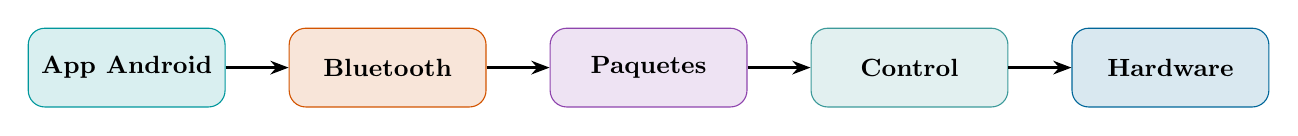
\begin{tikzpicture}[
		node distance=0.8cm,
		box/.style={
			draw,
			rounded corners=6pt,
			minimum width=2.5cm,
			minimum height=1cm,
			align=center,
			font=\small\bfseries
		},
		arrow/.style={-Stealth, thick}
		]
		
		\node[box, fill=arduinoTeal!15, draw=arduinoTeal] (android) {App Android};
		\node[box, fill=arduinoOrange!15, draw=arduinoOrange, right=of android] (bt) {Bluetooth};
		\node[box, fill=arduinoPurple!15, draw=arduinoPurple, right=of bt] (pkt) {Paquetes};
		\node[box, fill=arduinoLightGreen!15, draw=arduinoLightGreen, right=of pkt] (ctrl) {Control};
		\node[box, fill=arduinoBlue!15, draw=arduinoBlue, right=of ctrl] (hw) {Hardware};
		
		\draw[arrow] (android) -- (bt);
		\draw[arrow] (bt) -- (pkt);
		\draw[arrow] (pkt) -- (ctrl);
		\draw[arrow] (ctrl) -- (hw);
		
	\end{tikzpicture}
\end{center}

\section{Capa de Entrada (Telemetría Local de Sensores y Botones)}

\subsection{Propósito}

La capa de entrada permite que el ESP32 no solo actúe como receptor de comandos,
sino también como una \textbf{fuente de datos} para la aplicación Android.

Este módulo:
\begin{itemize}
	\item Lee sensores analógicos locales
	\item Lee botones y switches digitales
	\item Empaqueta los datos en una trama binaria de telemetría
	\item Envía los datos por Bluetooth hacia Android
\end{itemize}

Forma un canal de comunicación bidireccional donde tanto el teléfono como
el ESP32 pueden generar telemetría en tiempo real.

\subsection{Archivo de cabecera: \ardfnDG{input.h}}

\begin{lstlisting}
	#ifndef INPUT_H
	#define INPUT_H
	#include <Arduino.h>
	
	void inputInit();
	void inputUpdate();
	
	#endif
\end{lstlisting}

\subsection{Entradas soportadas}

\subsubsection{Entradas analógicas}

El ESP32 soporta canales ADC en pines de solo entrada:

\begin{center}
	\renewcommand{\arraystretch}{1.3}
	\setlength{\tabcolsep}{12pt}
	
	\begin{tabular}{@{} c c l @{}}
		\toprule
		\rowcolor{tableHeader!20}
		\textbf{GPIO} & \textbf{Canal ADC} & \textbf{Uso típico}  \\
		\midrule
		
		\rowcolor{rowGray}
		\multicolumn{3}{l}{\textbf{Entradas ADC}}                      \\
		
		34            & ADC1\_6              & Potenciómetro, sensor \\
		35            & ADC1\_7              & Potenciómetro, sensor \\
		36            & ADC1\_0              & Divisor de batería    \\
		39            & ADC1\_3              & Presión, temperatura  \\
		
		\bottomrule
	\end{tabular}
\end{center}

\subsubsection{Entradas digitales}
\begin{center}
	\renewcommand{\arraystretch}{1.3}
	\setlength{\tabcolsep}{12pt}
	
	\begin{tabular}{@{} c l @{}}
		\toprule
		\rowcolor{tableHeader!20}
		\textbf{GPIO} & \textbf{Uso}             \\
		\midrule
		
		\rowcolor{rowGray}
		\multicolumn{2}{l}{\textbf{Botones locales}} \\
		
		0             & Botón / selección de modo \\
		16            & Botón                     \\
		17            & Botón                     \\
		
		\bottomrule
	\end{tabular}
\end{center}

Todos los pines digitales usan el modo \texttt{INPUT\_PULLUP} y por lo tanto
leen LOW cuando están presionados.

\subsection{Formato del paquete}

La telemetría de entrada se empaqueta en la siguiente estructura binaria:

\begin{lstlisting}
	typedef struct {
		byte h1;      // 0xCC
		byte h2;      // 0x55
		uint16_t a34;
		uint16_t a35;
		uint16_t a36;
		uint16_t a39;
		byte d0;
		byte d16;
		byte d17;
		byte checksum;
	} InputPacket;
\end{lstlisting}

\subsection{Control de tiempo}

El paquete se envía cada:

\begin{lstlisting}
	const unsigned long inputInterval = 50; // ms
\end{lstlisting}

Esto crea un flujo de telemetría de 20 Hz.

\subsection{Inicialización}

\begin{lstlisting}
	void inputInit() {
		pinMode(PIN_D0,  INPUT_PULLUP);
		pinMode(PIN_D16, INPUT_PULLUP);
		pinMode(PIN_D17, INPUT_PULLUP);
		
		pinMode(PIN_A34, INPUT);
		pinMode(PIN_A35, INPUT);
		pinMode(PIN_A36, INPUT);
		pinMode(PIN_A39, INPUT);
	}
\end{lstlisting}

\subsection{Bucle principal de actualización}

\begin{lstlisting}
	void inputUpdate() {
		if (!SerialBT.hasClient()) return;
		if (millis() - lastSend < inputInterval) return;
		lastSend = millis();
	}
\end{lstlisting}

Esto asegura:
\begin{itemize}
	\item No hay transmisión cuando no hay un dispositivo Android conectado
	\item Uso de ancho de banda fijo y controlado
\end{itemize}

\subsection{Adquisición de datos}

\begin{lstlisting}[escapeinside={(*@}{@*)},]
	(*@\textcolor{arduinoOrange}{inputPacket}@*).(*@\textcolor{arduinoOrange}{a34}@*) = analogRead(PIN_A34);
	(*@\textcolor{arduinoOrange}{inputPacket}@*).(*@\textcolor{arduinoOrange}{a35}@*) = analogRead(PIN_A35);
	(*@\textcolor{arduinoOrange}{inputPacket}@*).(*@\textcolor{arduinoOrange}{a36}@*) = analogRead(PIN_A36);
	(*@\textcolor{arduinoOrange}{inputPacket}@*).(*@\textcolor{arduinoOrange}{a39}@*) = analogRead(PIN_A39);
	
	(*@\textcolor{arduinoOrange}{inputPacket}@*).(*@\textcolor{arduinoOrange}{d0}@*)  = !digitalRead(PIN_D0);
	(*@\textcolor{arduinoOrange}{inputPacket}@*).(*@\textcolor{arduinoOrange}{d16}@*) = !digitalRead(PIN_D16);
	(*@\textcolor{arduinoOrange}{inputPacket}@*).(*@\textcolor{arduinoOrange}{d17}@*) = !digitalRead(PIN_D17);
\end{lstlisting}

\subsection{Generación del checksum}

\begin{lstlisting}[escapeinside={(*@}{@*)},]
	byte c = 0;
	for (int i = 2; i < INPUT_PACKET_SIZE - 1; i++)
	c += ((byte*)&inputPacket)[i];
	
	(*@\textcolor{arduinoOrange}{inputPacket}@*).(*@\textcolor{arduinoOrange}{checksum}@*) = c;
\end{lstlisting}

\subsection{Transmisión}

\begin{lstlisting}
	SerialBT.write((byte*)&inputPacket, INPUT_PACKET_SIZE);
\end{lstlisting}

\subsection{Integración del sistema}

La capa de entrada completa el bucle total de telemetría:
\begin{center}
	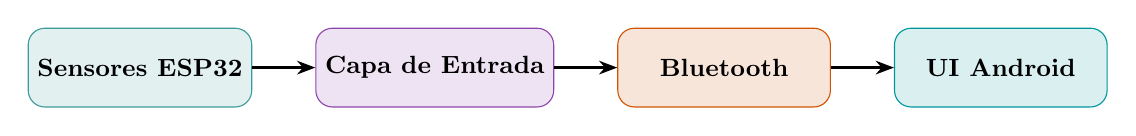
\begin{tikzpicture}[
		node distance=0.8cm,
		box/.style={
			draw,
			rounded corners=6pt,
			minimum width=2.7cm,
			minimum height=1cm,
			align=center,
			font=\small\bfseries
		},
		arrow/.style={-Stealth, thick}
		]
		
		\node[box, fill=arduinoLightGreen!15, draw=arduinoLightGreen] (sensors) {Sensores ESP32};
		\node[box, fill=arduinoPurple!15, draw=arduinoPurple, right=of sensors] (input) {Capa de Entrada};
		\node[box, fill=arduinoOrange!15, draw=arduinoOrange, right=of input] (bt) {Bluetooth};
		\node[box, fill=arduinoTeal!15, draw=arduinoTeal, right=of bt] (ui) {UI Android};
		
		\draw[arrow] (sensors) -- (input);
		\draw[arrow] (input) -- (bt);
		\draw[arrow] (bt) -- (ui);
		
	\end{tikzpicture}
\end{center}

Esto permite que Android muestre:
\begin{itemize}
	\item Voltaje de batería
	\item Datos de sensores externos
	\item Estados de botones físicos
\end{itemize}


\section{Capa de Telemetría de Sensores I2C}

\subsection{Propósito}

La capa de sensores I2C permite que el ESP32 lea sensores digitales externos y
transmita sus valores en tiempo real a la aplicación Android utilizando el mismo
canal de telemetría por Bluetooth.

Este módulo:
\begin{itemize}
	\item Inicializa el bus I2C
	\item Lee sensores de temperatura
	\item Lee unidades de medición inercial (IMU)
	\item Empaqueta los valores de los sensores en una trama de telemetría
	\item Envía el paquete a la aplicación Android
\end{itemize}

El módulo es \textbf{solo de escritura}: nunca interpreta datos entrantes.

\subsection{Interfaz pública: \ardfnDG{i2c\_sensors.h}}

\begin{lstlisting}
	void i2cInit();
	void sendI2CTelemetry();
\end{lstlisting}

\subsection{Configuración del bus I2C}

\begin{lstlisting}
	void i2cInit() {
		Wire.begin(21,22);
	}
\end{lstlisting}

\begin{itemize}
	\item GPIO 21 $\rightarrow$ SDA
	\item GPIO 22 $\rightarrow$ SCL
	\item Se requieren resistencias pull-up estándar para I2C
\end{itemize}

\subsection{Sensores soportados}

\subsubsection{Sensor de temperatura}

\begin{itemize}
	\item Dirección: \texttt{0x48}
	\item Registro de temperatura de 16 bits
\end{itemize}

\begin{lstlisting}
	uint16_t readTemp() {
		Wire.beginTransmission(I2C_ADDR_TEMP);
		Wire.write(0);
		Wire.endTransmission();
		Wire.requestFrom(I2C_ADDR_TEMP,2);
		return (Wire.read()<<8)|Wire.read();
	}
\end{lstlisting}

\subsubsection{IMU (acelerómetro)}

\begin{itemize}
	\item Dirección: \texttt{0x68}
	\item Registros: 0x3B–0x40 (AX, AY, AZ)
\end{itemize}

\begin{lstlisting}
	void readIMU(int16_t &ax,int16_t &ay,int16_t &az) {
		Wire.beginTransmission(I2C_ADDR_IMU);
		Wire.write(0x3B);
		Wire.endTransmission(false);
		Wire.requestFrom(I2C_ADDR_IMU,6);
		ax = (Wire.read()<<8)|Wire.read();
		ay = (Wire.read()<<8)|Wire.read();
		az = (Wire.read()<<8)|Wire.read();
	}
\end{lstlisting}

\subsection{Paquete de telemetría I2C}

\begin{lstlisting}
	typedef struct {
		byte h1;     // 0xCC
		byte h2;     // 0x66
		uint16_t temp;
		uint16_t ax;
		uint16_t ay;
		uint16_t az;
		byte sensorFlags;
		byte checksum;
	} I2CPacket;
\end{lstlisting}

\subsection{Frecuencia de transmisión}

\begin{lstlisting}
	const unsigned long i2cInterval = 100; // ms
\end{lstlisting}

Esto genera un flujo de telemetría de 10 Hz.

\subsection{Emisor de telemetría}

\begin{lstlisting}
	void sendI2CTelemetry() {
		if(!SerialBT.hasClient()) return;
		if(millis()-lastSend<i2cInterval) return;
		lastSend=millis();
	}
\end{lstlisting}

\subsection{Construcción del paquete}

\begin{lstlisting}[escapeinside={(*@}{@*)},]
	(*@\textcolor{arduinoOrange}{i2cPacket}@*).(*@\textcolor{arduinoOrange}{h1}@*)=0xCC;
	(*@\textcolor{arduinoOrange}{i2cPacket}@*).(*@\textcolor{arduinoOrange}{h2}@*)=0x66;
	(*@\textcolor{arduinoOrange}{i2cPacket}@*).(*@\textcolor{arduinoOrange}{temp}@*) = readTemp();
	readIMU(ax,ay,az);
	
	(*@\textcolor{arduinoOrange}{i2cPacket}@*).(*@\textcolor{arduinoOrange}{ax}@*)=ax;
	(*@\textcolor{arduinoOrange}{i2cPacket}@*).(*@\textcolor{arduinoOrange}{ay}@*)=ay;
	(*@\textcolor{arduinoOrange}{i2cPacket}@*).(*@\textcolor{arduinoOrange}{az}@*)=az;
	(*@\textcolor{arduinoOrange}{i2cPacket}@*).(*@\textcolor{arduinoOrange}{sensorFlags}@*)=0b00000011;
\end{lstlisting}

\subsection{Checksum y transmisión}

\begin{lstlisting}[escapeinside={(*@}{@*)},]
	byte c=0;
	for(int i=2;i<I2C_PACKET_SIZE-1;i++)
	c+=((byte*)&i2cPacket)[i];
	
	(*@\textcolor{arduinoOrange}{i2cPacket}@*).(*@\textcolor{arduinoOrange}{checksum}@*)=c;
	SerialBT.write((byte*)&i2cPacket,I2C_PACKET_SIZE);
\end{lstlisting}

\subsection{Integración del sistema}

\begin{center}
	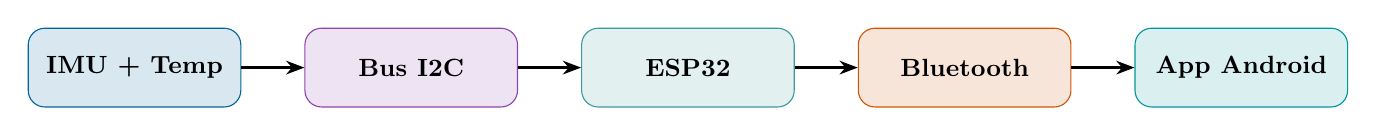
\begin{tikzpicture}[
		node distance=0.8cm,
		box/.style={
			draw,
			rounded corners=6pt,
			minimum width=2.7cm,
			minimum height=1cm,
			align=center,
			font=\small\bfseries
		},
		arrow/.style={-Stealth, thick}
		]
		
		\node[box, fill=arduinoBlue!15, draw=arduinoBlue] (imu) {IMU + Temp};
		\node[box, fill=arduinoPurple!15, draw=arduinoPurple, right=of imu] (i2c) {Bus I2C};
		\node[box, fill=arduinoLightGreen!15, draw=arduinoLightGreen, right=of i2c] (esp) {ESP32};
		\node[box, fill=arduinoOrange!15, draw=arduinoOrange, right=of esp] (bt) {Bluetooth};
		\node[box, fill=arduinoTeal!15, draw=arduinoTeal, right=of bt] (app) {App Android};
		
		\draw[arrow] (imu) -- (i2c);
		\draw[arrow] (i2c) -- (esp);
		\draw[arrow] (esp) -- (bt);
		\draw[arrow] (bt) -- (app);
		
	\end{tikzpicture}
\end{center}

Esto permite mostrar en tiempo real:
\begin{itemize}
	\item Temperatura de la placa
	\item Aceleración del vehículo
	\item Detección de movimiento
\end{itemize}

\section{Capa de Depuración y Diagnóstico}

\subsection{Propósito}

La Capa de Depuración centraliza toda la salida formateada por
\texttt{Serial} que se utiliza para monitorear, probar y validar
el sistema de comunicación.

Este módulo:

\begin{itemize}
	\item Decodifica campos binarios de los paquetes en texto legible
	\item Imprime los valores en un formato claro y fácil de interpretar
	\item Mantiene la lógica de depuración separada de la lógica de control
\end{itemize}

Este módulo \textbf{nunca} se comunica por Bluetooth y \textbf{nunca} modifica
los datos. Solo lee las estructuras globales de paquetes.

\subsection{Archivo de Cabecera: \ardfnDG{debug.h}}

\begin{lstlisting}
	#ifndef DEBUG_H
	#define DEBUG_H
	
	#include <Arduino.h>
	#include "packets.h"
	
	void printStatePacket();
	void printEventPacket();
	void printPanelPacket();
	void printIndicatorPacket();
	void printPlotPacket();
	
	#endif
\end{lstlisting}

\subsection{Archivo de Implementación: \ardfnDG{debug.cpp}}

\subsubsection{Impresor de Paquetes de Estado}

\begin{lstlisting}[escapeinside={(*@}{@*)}]
	void printStatePacket() {
		Serial.println("\n--- RC STATE PACKET ---");
		
		Serial.printf("L Stick: X=%u  Y=%u\n",
		(*@\textcolor{arduinoOrange}{rcStatePacket}@*).(*@\textcolor{arduinoOrange}{data}@*).(*@\textcolor{arduinoOrange}{leftStickX}@*),
		(*@\textcolor{arduinoOrange}{rcStatePacket}@*).(*@\textcolor{arduinoOrange}{data}@*).(*@\textcolor{arduinoOrange}{leftStickY}@*));
		
		Serial.printf("R Stick: X=%u  Y=%u\n",
		(*@\textcolor{arduinoOrange}{rcStatePacket}@*).(*@\textcolor{arduinoOrange}{data}@*).(*@\textcolor{arduinoOrange}{rightStickX}@*),
		(*@\textcolor{arduinoOrange}{rcStatePacket}@*).(*@\textcolor{arduinoOrange}{data}@*).(*@\textcolor{arduinoOrange}{rightStickY}@*));
		
		Serial.printf("Knobs:   L=%u  R=%u\n",
		(*@\textcolor{arduinoOrange}{rcStatePacket}@*).(*@\textcolor{arduinoOrange}{data}@*).(*@\textcolor{arduinoOrange}{leftKnob}@*),
		(*@\textcolor{arduinoOrange}{rcStatePacket}@*).(*@\textcolor{arduinoOrange}{data}@*).(*@\textcolor{arduinoOrange}{rightKnob}@*));
		
		byte s = (*@\textcolor{arduinoOrange}{rcStatePacket}@*).(*@\textcolor{arduinoOrange}{data}@*).(*@\textcolor{arduinoOrange}{switches}@*);
		Serial.printf("Switch Byte: 0x%02X\n", s);
		
		for (int i = 0; i < 6; i++) {
			Serial.printf(
			"  S%d = %s\n",
			i + 1,
			(s & (1 << i)) ? "ON" : "OFF"
			);
		}
		
		Serial.printf("Checksum: %u\n",
		(*@\textcolor{arduinoOrange}{rcStatePacket}@*).(*@\textcolor{arduinoOrange}{data}@*).(*@\textcolor{arduinoOrange}{checksum}@*));
		
		Serial.println("------------------------");
	}
\end{lstlisting}

\subsubsection{Impresor de Paquetes de Evento}

\begin{lstlisting}[escapeinside={(*@}{@*)}]
	void printEventPacket() {
		Serial.println("\n--- EVENT PACKET ---");
		Serial.printf("Event ID: 0x%02X\n",
		(*@\textcolor{arduinoOrange}{rcEventPacket}@*).(*@\textcolor{arduinoOrange}{data}@*).(*@\textcolor{arduinoOrange}{eventId}@*));
		Serial.printf("Checksum: 0x%02X\n",
		(*@\textcolor{arduinoOrange}{rcEventPacket}@*).(*@\textcolor{arduinoOrange}{data}@*).(*@\textcolor{arduinoOrange}{checksum}@*));
		Serial.println("---------------------");
	}
\end{lstlisting}

\subsubsection{Impresor de Telemetría del Panel}

\begin{lstlisting}[escapeinside={(*@}{@*)}]
	void printPanelPacket() {
		Serial.println("\n--- PANEL TELEMETRY ---");
		Serial.printf("Left: %u  Right: %u\n",
		(*@\textcolor{arduinoOrange}{panelPacket}@*).(*@\textcolor{arduinoOrange}{leftPanelValue}@*),
		(*@\textcolor{arduinoOrange}{panelPacket}@*).(*@\textcolor{arduinoOrange}{rightPanelValue}@*));
		Serial.printf("States: 0x%02X\n",
		(*@\textcolor{arduinoOrange}{panelPacket}@*).(*@\textcolor{arduinoOrange}{panelStates}@*));
		Serial.printf("Checksum: %u\n",
		(*@\textcolor{arduinoOrange}{panelPacket}@*).(*@\textcolor{arduinoOrange}{checksum}@*));
	}
\end{lstlisting}

\subsubsection{Impresor de Telemetría de Indicadores}

\begin{lstlisting}[escapeinside={(*@}{@*)}]
	void printIndicatorPacket() {
		Serial.println("\n--- INDICATOR TELEMETRY ---");
		Serial.printf("Analog: %u\n",
		(*@\textcolor{arduinoOrange}{indicatorPacket}@*).(*@\textcolor{arduinoOrange}{analogValue}@*));
		Serial.printf("Battery: %u%%\n",
		(*@\textcolor{arduinoOrange}{indicatorPacket}@*).(*@\textcolor{arduinoOrange}{batteryLevel}@*));
		Serial.printf("Checksum: %u\n",
		(*@\textcolor{arduinoOrange}{indicatorPacket}@*).(*@\textcolor{arduinoOrange}{checksum}@*));
	}
\end{lstlisting}

\subsubsection{Impresor de Telemetría de Gráficas}

\begin{lstlisting}[escapeinside={(*@}{@*)}]
	void printPlotPacket() {
		Serial.println("\n--- PLOT TELEMETRY ---");
		Serial.printf("Plots: %u\n",
		(*@\textcolor{arduinoOrange}{plotPacket}@*).(*@\textcolor{arduinoOrange}{numPlots}@*));
		Serial.printf("P1=%u  P2=%u  P3=%u\n",
		(*@\textcolor{arduinoOrange}{plotPacket}@*).(*@\textcolor{arduinoOrange}{plotValue1}@*),
		(*@\textcolor{arduinoOrange}{plotPacket}@*).(*@\textcolor{arduinoOrange}{plotValue2}@*),
		(*@\textcolor{arduinoOrange}{plotPacket}@*).(*@\textcolor{arduinoOrange}{plotValue3}@*));
		Serial.printf("Checksum: %u\n",
		(*@\textcolor{arduinoOrange}{plotPacket}@*).(*@\textcolor{arduinoOrange}{checksum}@*));
	}
\end{lstlisting}

\subsection{¿Por qué una Capa de Depuración Dedicada?}

\begin{itemize}
	\item Mantiene el código de control y telemetría limpio
	\item Permite habilitar o deshabilitar fácilmente los mensajes por Serial
	\item Evita problemas de temporización en la lógica Bluetooth
	\item Ayuda a visualizar estructuras de datos binarias
\end{itemize}
\end{document}